\section{Recepção de novatos e as Editatonas}

Desde sua criação, a Wikipédia viu seu número de usuários ativos crescer ano após ano. Isso era verdade até 2007, quando a tendência de crescimento desacelera e então a comunidade passa a encolher.  \citep{halfaker_rise_2013}

Essa afirmação, muito repetida na literatura wikipedista, é referente à versão anglófona da Wikipédia, que em Maio de 2007 teve um pico de 63.931 usuários ativos, seguido de praticamente uma década de declínio, até uma certa estabilização a partir de 2017 flutuando desde então em número em torno de 37 mil ativos por mês. \citep{wikimedia_stats_active_editors_enwiki_2020}

\begin{figure}[hbt]
    \centering
    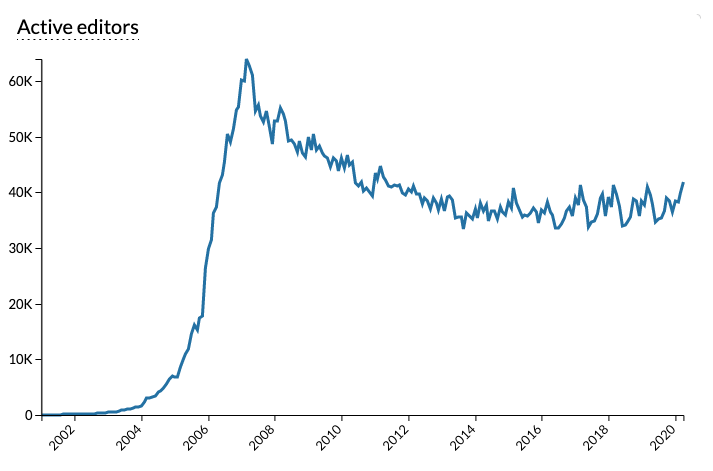
\includegraphics[width=1\textwidth]{Images/active_editors_enwiki.png}
    \caption{Número de usuários ativos na Wikipédia em inglês por mês. \citep{wikimedia_stats_active_editors_enwiki_2020} }
    \label{fig:active_editors_enwiki}
\end{figure}

Já a Wikipédia em português tem uma trajetória distinta de usuários ativos ao longo do tempo. Em maio de 2007, seu número de usuários ativos continuava a crescer, chegando no início do ano seguinte pela primeira vez à marca de 2 mil editores ativos por mês. \citep{wikimedia_stats_active_editors_ptwiki_2020}

Desde o pico de usuário ativos na Wikipédia em português até os dias de hoje podemos também observar um pequeno declínio, mas nada comparado ao vivenciado por sua irmã anglófona. Tirando uma vertiginosa queda de quase 25\% no número de usuários ativos durante a crise do CAPTCHA (narrada no capítulo anterior), o número de usuários ativos se em português vem se mantendo após isso razoavelmente estável em uma flutuação em torno de 1700 por mês.

\begin{figure}[hbt]
    \centering
    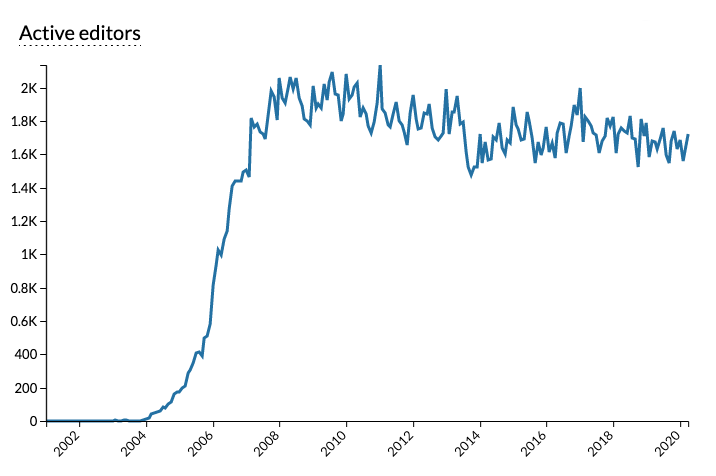
\includegraphics[width=1\textwidth]{Images/active_editors_ptwiki.png}
    \caption{Número de usuários ativos na Wikipédia em inglês por mês. \citep{wikimedia_stats_active_editors_ptwiki_2020} }
    \label{fig:active_editors_ptwiki}
\end{figure}

Se por um lado a análise bruta dos dados de engajamento na atividade de escrita nas Wikipédias não encontrou na versão em português o declínio apontando em sua versão principal, ela parece ao menos apontar que o crescimento orgânico da comunidade encontrou um teto. Isso foi notado pela comunidade, que entende precisar retomar o crescimento de seus membros ativos para ser capaz cumprir seu objetivo de ``disponibilizar todo conhecimento do mundo'' e para ter disponibilidade de mão de obra para garantir seus trabalhos administrativos. \citep{morgan_tea_2013}

Como dito por \cite{faulkner_etiquette_2012}: ``\textit{Atualmente, o maior desafio encarado pela comunidade da Wikipédia envolve (...) garantir que os colaboradores da enciclopédia continuem suficientemente numerosos para cumprir os papéis que a mantém relevante.}''\footnote{Tradução livre do original ``Currently, the greatest challenge faced by the Wikipedia community involves (...) ensuring that the encyclopedia’s contributors remain sufficiently numerous to fill the roles that keep it relevant.''}

Além das preocupações mais rasas e óbvias com os problemas ocasionados pela falta de oferta de mão de obra voluntária, existe no não crescimento da comunidade um problema conceitual que se defronta com a missão da Wikipédia: se é entendido que todo conhecimento tem um viés de acordo com quem o produz, a enciclopédia só poderá alcançar seu objetivo de reunir todo o conhecimento humano se todas as pessoas do mundo estiverem a editando. Somente assim ela poderia ter toda a diversidade humana representada.

É evidente que este enunciado é uma hipérbole, mas ele exerce a função de um norte utópico a ser buscado no fazer diário dos wikipedistas, e os mobiliza para pensar em formas de nortear sua ação rumo a esse objetivo. Seguindo esta bússola, diversos wikipedistas ativos se preocupam constantemente em pensar estratégias para reter novos usuários que se aproximem da enciclopédia. \citep{faulkner_etiquette_2012}, \citep{suh_singularity_2009}, \citep{musicant_mentoring_2011}, \citep{narayan_wikipedia_2017}.

Para além da Wikipédia, é conhecida pela literatura a dificuldade de entrada de neófitos em uma comunidade de prática. ``A ampla aceitação de artefatos e arranjos organizacionais é condição sine qua non para participar de uma comunidade de prática'' (Lave and Wenger 1991, Star 1996 apud \cite{feitosa_cidadao_2010}). Porém, estes artefatos e arranjos não são perfeitamente documentados (e nem haveria como serem por sua própria dinâmica de constante reconfiguração ao fazer), e sua descoberta e apropriação pode ser uma tarefa inglória para um inexperiente novato.

Como pode ser visto em \citep{steinmacher_social_2015}, essas dificuldades de entrada estão presentes tanto em comunidade de produção de código-fonte, como de artefatos culturais, como uma enciclopédia.

Falando especificamente da Wikipédia, esse cenário é agravado porque ``novos usuários da Wikipédia são desproporcionalmente afetados pelos mecanismos de controle de qualidade projetados para impedir spammers e publicidades'' \citep{schneider_accept_2014} \footnote{Tradução livre de ``new Wikipedia users are disproportionately affected by the quality assur- ance mechanisms designed to thwart spammers and promoters.''}, fazendo com que a missão de se tornar um contribuinte ativo da Wikipédia se torne ainda mais complexa do que em demais comunidades virtuais menos mediadas por ferramentas como as detalhadas no capítulo anterior.

Assim, sabendo que ``mensagens de boas vindas, assistência técnica e crítica construtiva com o tempo retardam o declínio natural nas edições dos novatos'' \citep{choi_socialization_2010}\footnote{Tradução livre de ``welcome messages, technical assistance, and constructive criticism over time retarded the natural decline in newcomers’ editing.''}, buscando se antecipar aos comuns percalços encontrados online para melhorar a forma como novatos chegam à Wikipédia e almejando com isso aumentar os índices de retenção futura destes usuários, wikipedistas experientes começam um momento que podemos chamar de  ``quando os de dentro saem''. Em um movimento análogo ao feito por cientistas, que devem sair fisicamente de seus laboratórios para fazer/reforçar enredamentos que irão manter/expandir a sua atuação \citep{latour_ciencia_1987}, os wikipedistas então passam a organizar as chamadas atividades de \textit{outreach}\footnote{Em uma tradução livre ao português poderíamos chamar essas atividades de extensionistas, mas a comunidade lusófona da Wikipédia utiliza em seu cotiano o termo \textit{outreach} em inglês mesmo, portanto seguiremos o utilizando desta forma na pesquisa.}. 

As ações de \textit{outreach} são um esforço ativo de fazer ``comunicação sobre a comunidade fora da comunidade'' e ``é especialmente importante para o recrutamento de potenciais novos membros. Recrutamento ativo ou invés de passivo, e comunicação focada naqueles que tem o perfil da comunidade, trará mais recrutas''\citep[p.37/38]{kraut_dealing_2010}. \footnote{Tradução livre do inglês: ``communication about the community outside the community. These are especially important to the recruitment of potential new members. Active rather than passive recruiting, and targeting communication to those who are a good fit to the community, will bring in more recruits.''}

Nestas atividades de outreach, editores experientes buscam aproximar as comunidades wikipedistas de outras comunidades e pessoas não engajadas diretamente. Essas atividades vão deste a realização de apresentações em escolas, universidade e em eventos de movimentos sociais que abram suas portas (muito corriqueiramente movimentos de software livre e feministas\citep{farzan_bring_2016}), à criação de estratégias para utilização em sala de aula da Wikipédia por professores, com wikipedistas atuando como voluntários no campus, \citep{marques_trabalhando_2012} até a realização de parcerias com instituições culturais GLAM, que podem contar com um ``wikipedista residente'' para atuar junto das equipes das instituições na produção de conteúdos enciclopédicos a partir de seus acervos. \citep{stinson_stepping_2018}

Dentro das diversas frentes de outreach, uma das principais estratégias do Movimento Wikimedia para engajar e trazer novos/as usuários/as à comunidade são as editatonas. Realizadas por todo o mundo, são eventos onde pessoas se reúnem para editar sobre um mesmo tema de interesse \citep{littlejohn_learning_2019}. Como definido pela própria enciclopédia, no verbete ``Maratona de edição'' na Wikipédia em português, uma editatona é um evento ``\textit{durante o qual editores se reúnem para editar e melhorar um tema ou tipo específico de conteúdo, geralmente incluindo um treinamento em edição básica para novos editores. A palavra é uma combinação das palavras ``editar'' (\textit{edit}) e ``maratona'' (\textit{marathon})}'' \citewiki{ptwiki_maratona}.

Em sua origem na língua inglesa, a palavra é grafada \textit{edit-a-thon} apresentando uma ambivalência, que é traída quando a traduzimos para o português. ``\textit{A ton}'' é uma forma anglófona de dizer "muito". Então, em sua origem, o nome do evento pode ser entendido além de ``maratona de edição'' também como simplesmente ``editar muito''. Mas, mesmo perdendo este significado adicional original, o nome editatona se estabelece nas comunidades lusófonas.

As editatonas são atividades quase onipresentes nas diversas formas de outreach do Movimento Wikimedia. Seja em parcerias GLAM, \citep{robichaud_wikipedia_2017} dentro do Programa de Educação \citep{marques_wikipedia_2013} ou em participações avulsas de wikipedistas em eventos diversos\citep{campany_using_2018}, é praticamente garantida a realização de uma editatona.

\begin{figure}[H]
    \centering
    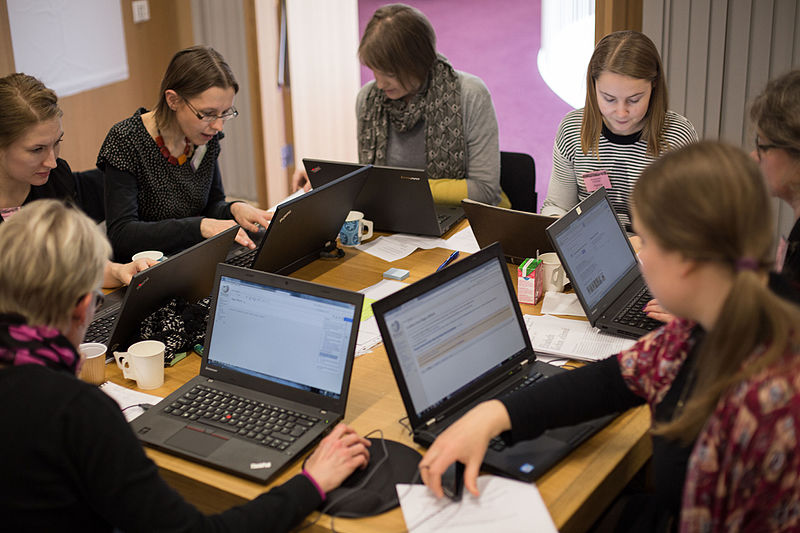
\includegraphics[width=1\textwidth]{Images/editatona_antiga.jpg}
    \caption{Exemplo de uma editatona presencial sendo realizada.}
    \label{fig:editatona_antiga}
\end{figure}

Há variações em seu formato, mas normalmente uma editatona começa com um (ou mais) editor/a(es/as) experiente(s) apresentando o funcionamento da enciclopédia e introduzindo suas políticas editoriais. Em sequência, os/as demais participantes começam a escrever, individualmente ou em grupo verbetes de seu interesse. Nesta fase, o/a(s) usuário/a(s) experiente(s) atua(m) como tutor/a(es/as), tirando dúvidas dos/as novatos/as que apareçam durante o processo de edição.

Existem também algumas editatonas que funcionam como ``forças-tarefas'' de usuários experientes melhorando verbetes sobre um determinado assunto focal, como por exemplo ``patrimônio natural brasileiro''\footnote{https://pt.wikipedia.org/wiki/Wikipédia:Edit-a-thon/Atividades\_em\_português/Wiki\_Loves\_Earth\_Brasil\_2015 , acessada em 19 de março de 2020.} ou ``eleições no Brasil''\footnote{https://meta.wikimedia.org/wiki/Programa\_Catalisador\_do\_Brasil/2013-2014/Micro-subsídios/Solicitação/Wikitona\_Eleições\_2014 , acessada em 19 de março de 2020.}. Estas atividades dispensam a explanação inicial, e, os/as presentes, editores/as já experientes, partem rapidamente para a divisão de tarefas e escrita de conteúdos. Habitualmente, essas forças tarefas são realizadas online, e a maioria das editatonas presenciais é direcionada em apresentar o mundo wiki a novos/as editores/as a partir de assuntos que sejam de seu interesse.

No início de 2020, a página para divulgação de editatonas da Wikipédia em português já contava com 120 eventos cadastrados desde 2013, sendo 115 deles (98,5\%) realizados no Brasil\citewiki{ptwiki_edit_a_thon_atividades_portugues}. Já na página para editatonas da Wikipédia em inglês, estavam mapeados 121 eventos, com o primeiro datando de janeiro de 2011 e o último de maio de 2018\citewiki{enwiki_how_run_edit_a_thon}, indicando que provavelmente essa comunidade passou a registrar seus eventos realizados no último ano e meio em outro lugar. Já a Wikipédia em espanhol apresentava 92 eventos\citewiki{eswiki_editaton}, mas aparentemente México, Argentina e Espanha, pólos movimentados de atividade wiki, estão com seus números desatualizados. Terminando nosso passeio pelas páginas sobre editatonas das maiores Wikipédias do mundo, encontramos 60 atividades mapeadas na versão francófona (com destaque para um evento realizado recentemente em Guiné, o primeiro fora do eixo França-Canadá)\citewiki{frwiki_journées_contributives} e 83 na enciclopédia em alemão\citewiki{dewiki_edit_a_thon}.

Se por um lado nossa breve busca não conseguiu números precisos sobre a quantidade de editatonas realizadas pelo mundo, entendemos que os valores encontrados já são suficientes para chancelar a relevância deste tipo de evento para o Movimento Wikimedia. Esses dados também indicam que, além da organização destes eventos ser uma estratégia muito utilizada por todo o mundo, ela é especialmente popular no Brasil. Com essa constatação, elegemos então as editatonas como o método a ser acompanhado por nossa pesquisa para observar \textit{in loco} a chega de novos usuários à enciclopédia.
